\chapter[Metodologia do projeto]{METODOLOGIA DO PROJETO}

Nesta capítulo será definido a metodologia utilizado no projeto, definindo cada papel e atividade que será realizada ao longo do projeto.

\section{Metodologias Ágeis}

No começo dos anos 90 começou-se uma nova maneira de produzir software, e essa nova metodologia era mais centrada na qualidade do produto entregue e na satisfação do usuário. Esta nova abordagem ficou conhecida como ágil.

Para um melhor aproveitamento do projeto será utilizado duas metodologias já conhecidas para o desenvolvimento de projetos de software como o \textit{SCRUM} e o \textit{SAFe}, porém com adaptações para que possa ser utilizada no projeto proposto. Além do uso de ferramentas de gerenciamento como os \textit{Kanbans}.

\subsection{Kanban}

Kanban é uma ferramenta de apoio ao gerenciamento de projetos. É possível acompanhar tarefas que são planejadas e priorizadas mas que estão pendentes, tarefas em andamento e as que já foram concluídas. A ferramenta tem um formato de quadro com abas para cada estágio de conclusão da atividade e cada atividade é descrita por meio de cartões que são arrastados pelas abas do quadro.

Além do formato manual, que pode ser realizado com post-its e um quadro branco ou cartolinas, existem ferramentas automatizadas do Kanban, como o software \textit{Trello}. Para o gerenciamento das atividades de cada membro da equipe será utilizado o \textit{Trello}. Nele é possível atribuir a tarefa a determinado membro e ter uma visão geral do que está sendo feito e quem é o responsável por concluir determinada tarefa.
O \textit{Kanban} também pode ser utilizado por um repositório dentro do Github, por meio do Zenhub, onde acontece o controle de versão de código pela equipe de software por conta de ter um melhor gerenciamento com o versionamento. A partir da priorização da e atribuição de pontos a cada \textit{User Story}, essas informações são sincronizadas no Kanban e assim a equipe acompanha o desenvolvimento do software ao longo da Sprint.


\subsection{Adaptação SCRUM e SAFe}

\begin{figure}[ht]
	\centering
    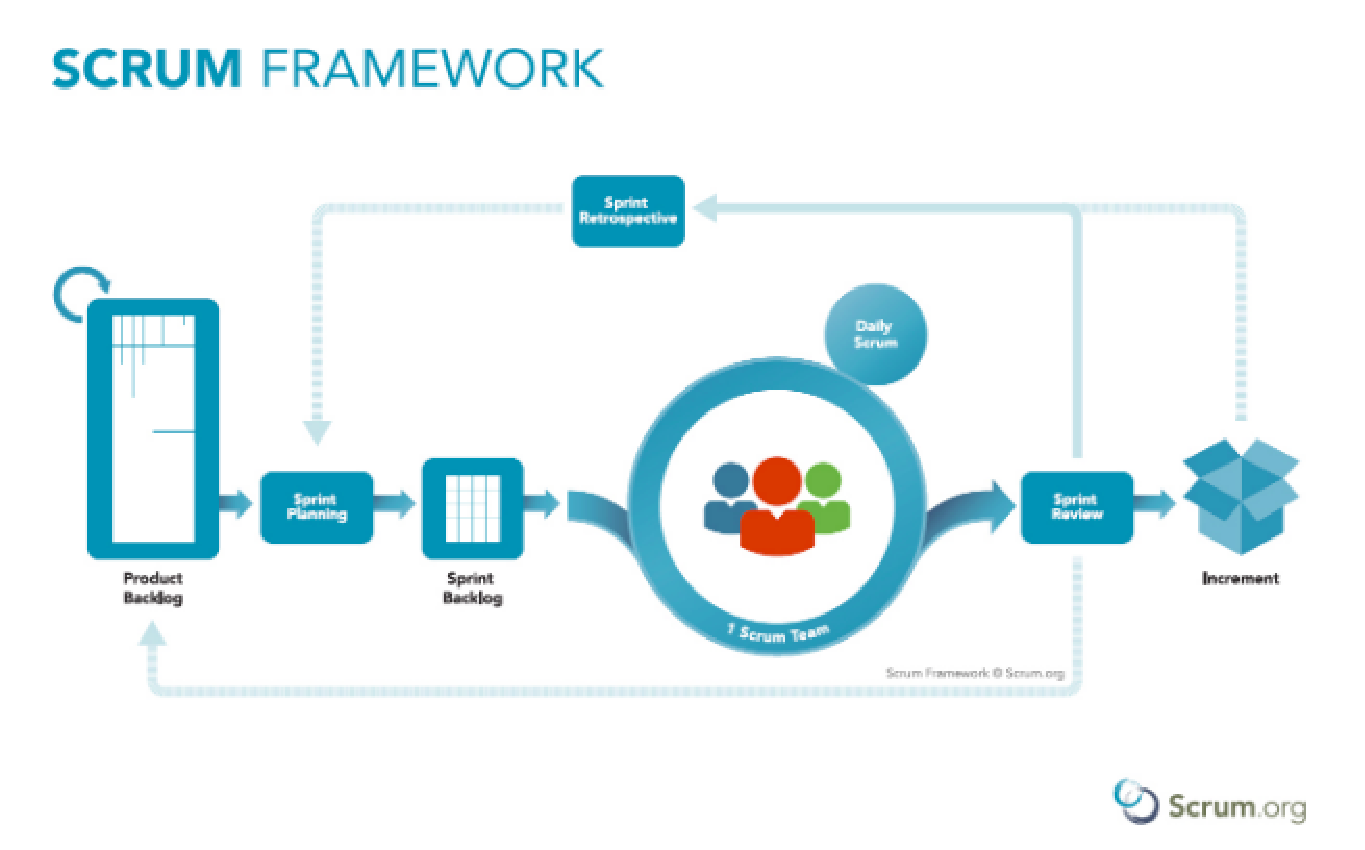
\includegraphics[keepaspectratio=true,scale=0.7]{figuras/scrum.eps}
    \caption[SCRUM.]{SCRUM. Fonte: Scrum.org}
	\label{fig:scrum}
\end{figure}

Scrum é uma metodologia ágil nos quais os projetos são divididos em ciclos, esses ciclos são definidos pela equipe, e elas se chamam \textit{sprints}. Uma sprint define um intervalo de tempo em que um conjunto de funcionalidades e atividades devem ser executados. No nosso caso ela será semanal.

A lista de funcionalidades e atividades listadas pela equipe se chama \textit{Product Backlog}. No início de cada \textit{sprint} é feito uma reunião, que recebe o nome de \textit{Sprint Planning}, na qual irá priorizar uma lista de funcionalidades que serão entregues naquele espaço de tempo, respeitando a importância de cada funcionalidade.

Todos as quartas e sextas a equipe se reúne para fazer uma breve reunião, que recebe o nome de \textit{Daily Meeting}, e tem como objetivo informar a situação do que se está fazendo, se existe algum impedimento.

No final de cada sprint, que se chama \textit{Sprint Review}, a equipe apresenta tudo que foi feito durante aquele período de tempo, faz a integração de todas as partes e planeja a próxima \textit{sprint}.

Na metodologia Scrum também existem papéis, e estes são:

\begin{itemize}
    \item \textbf{Scrum Master}: É o responsável por garantir que o projeto ocorra de maneira eficiente removendo os empecilhos que possam vir a atrapalhar a equipe. Garante que os rituais do \textit{Scrum} sejam aplicados corretamente. Esse papel no projeto será monitorado pelo \textbf{coordenador geral} e seus \textbf{diretores técnicos}.
    \item \textbf{Product owner}: Fornece o conhecimento do negócio e traduz para requisitos as necessidades do projeto, assim como a ordem de aplicação. Ele também é quem faz a validação das funcionalidades que foram desenvolvidas. Esse papel no projeto será desempenhado pelo \textbf{Diretor de Qualidade}.
    \item \textbf{Desenvolvedores}: Responsável pelo desenvolvimento do produto. Os desenvolvedores são capazes de mensurar a complexidade de uma \textit{User Story}.
\end{itemize}

A organização do processo foi feito utilizando as boas práticas definidas no SAFe que separa o processo inteiro em 3 grandes níveis, são eles: Portfólio, Programa e Time. O nível de portfólio é responsável por boa parte da documentação do projeto e modelagens. O nível de programa é onde será definido a arquitetura e toda a estrutura que precisar para que o time possa começar a trabalhar. O último nível é o de time que é onde a solução é desenvolvida.

O processo da figura \ref{fig:requisitos} e figura \ref{fig:desenvolvimento} exemplifica a adaptação que utilizamos das metodologias \textit{SCRUM} e \textit{SAFe} em um processo enxuto que será aplicado no projeto:

\subsection{Processo de engenharia de requisitos}

\begin{figure}[ht]
	\centering
    \includegraphics[keepaspectratio=true,scale=0.5]{figuras/desenvolvimento.eps}
    \caption[Processo de engenharia de requisitos.]{Processo de engenharia de requisitos. Fonte: Autor}
	\label{fig:requisitos}
\end{figure}

Na engenharia de requisitos é iniciada na etapa de elicitação com a identificação do problema e do contexto com isso é definido um tema de investimento. Esse tema será mapeado em features e enables que são seus requisitos funcionais e não funcionais respectivamente. Na etapa de modelagem será feito um pequeno diagrama funcional e não funcional de forma incremental do projeto. Por fim na fase de análise será feito os planos de gerenciamento de risco, tempo, custo e recursos humanos além do termo de abertura de projeto.

\subsection{Processo de desenvolvimento}

\begin{figure}[ht]
	\centering
    \includegraphics[keepaspectratio=true,scale=0.5]{figuras/desenvolvimento.eps}
    \caption[Processo de desenvolvimento.]{Processo de desenvolvimento. Fonte: Autor}
	\label{fig:desenvolvimento}
\end{figure}

Finalizado o subprocesso de engenharia de requisitos partiremos para o processo de desenvolvimento, inicialmente será definido a arquitetura e o product backlog com isso o time de desenvolvimento irá dar início as atividades para a finalização do projeto. O projeto é iterativo e incremental, ou seja, de acordo com as necessidades do projeto o ciclo pode se repetir várias vezes o que chamamos de Sprints.